\documentclass[a4paper,10pt]{article}

\usepackage[margin=1.2cm]{geometry}
\usepackage{ucs}
\usepackage[utf8]{inputenc}
\usepackage{amsmath}
\usepackage{caption}
\usepackage{subcaption}
\usepackage{graphicx}
% \usepackage{subfigure}
\usepackage{xcolor}
\usepackage[english]{babel}
\usepackage{fontenc}
\usepackage{graphicx}
% \usepackage{mathtools}
\usepackage{siunitx}
\setlength\parindent{0pt}
% \usepackage{psbox}
% \usepackage{auto-pst-pdf}
\usepackage{tikz}
\usetikzlibrary{arrows.meta}

\usepackage{hyperref}

\author{Ömer Faruk Birgül}
% \title{Homework 5}
\title{Homework 7 \\ \large Realizing a Given Boolean Function and Constructing the Optimum Layout}
% \subtitle{Inverter Delay}
\date{\today}

\begin{document}
\maketitle
\section{Schematic}
% I used KiCad \& ngspice to simulate inverter. KiCad is normally PCB drawing program but it has simulation capability by using ngspice. I also used ChatGPT to create Python scripts to draw waveforms. Datas of these waveforms are generated by KiCad.
\autoref{fig:sch} shows schematic of the circuit and nodes are marked to use them to generate Euler's Path
\begin{figure}[ht!]
 \centering
 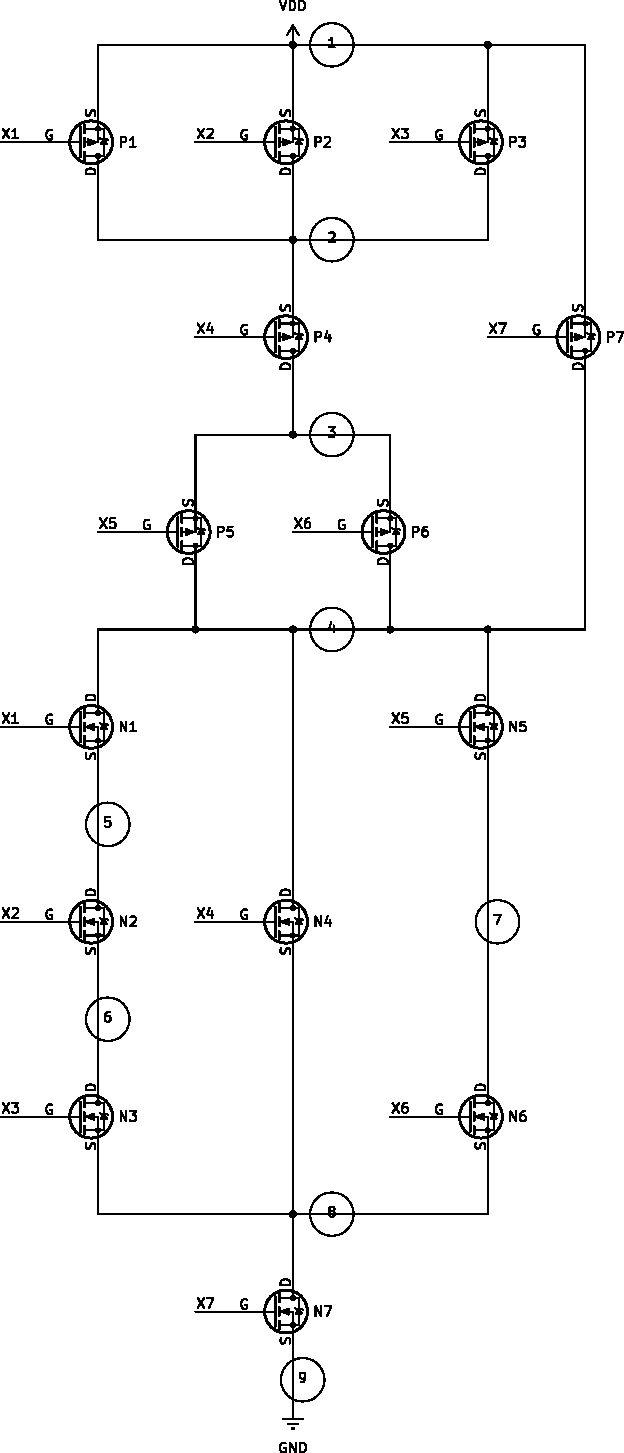
\includegraphics[width=0.4\textwidth]{output_nodes_small.pdf}

 \caption{Circuit schematic with marked nodes.}
  \label{fig:sch}
\end{figure}

\newpage
\section{Euler's Path}
\autoref{fig:euler_pmos} shows PMOS part of the network and \autoref{fig:euler_nmos} shows NMOS part of the network. In both graphs, $(start)$ shows start node, and $(stop)$ shows stop node. And arrows shows to path for following. When we follow paths, it gives X5-X6-X4-X1-X2-X3-X7. This is our common Euler Path.


\begin{figure}[!ht]
\centering
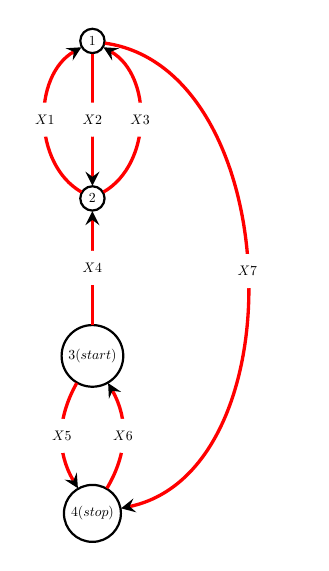
\begin{tikzpicture}[scale=0.5, transform shape]
\begin{scope}[every node/.style={circle,thick,draw}]
    \node (1) at (0,0) {$1$};
    \node (2) at (0,-4) {$2$};
    \node (3) at (0,-8) {$3(start)$};
    \node (4) at (0,-12) {$4(stop)$};
\end{scope}
\begin{scope}[>={stealth[black]}, every node/.style={fill=white,circle}, every edge/.style={draw=red,very thick}]

    \path [->] (2) edge[bend left=60] node {$X1$} (1);
    \path [->] (1) edge node {$X2$} (2);
    \path [->] (2) edge[bend right=60] node {$X3$} (1);
    \path [->] (3) edge node {$X4$} (2);
    \path [->] (3) edge[bend right=30] node {$X5$} (4);
    \path [->] (4) edge[bend right=30] node {$X6$} (3);
    \path [->] (1) edge[bend left=80] node {$X7$} (4);
\end{scope}
\end{tikzpicture}
\caption{pMOS Network Graph}
\label{fig:euler_pmos}
\end{figure}

\begin{figure}[!ht]
\centering
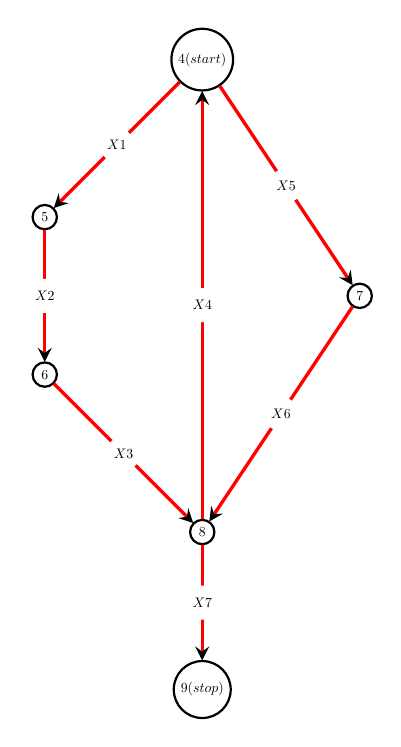
\begin{tikzpicture}[scale=0.5, transform shape]
\begin{scope}[every node/.style={circle,thick,draw}]
    \node (4) at (0,0) {$4(start)$};
    \node (5) at (-4,-4) {$5$};
    \node (6) at (-4,-8) {$6$};
    \node (7) at (4,-6) {$7$};
    \node (8) at (0,-12) {$8$};
    \node (9) at (0,-16) {$9(stop)$} ;
\end{scope}
\begin{scope}[>={stealth[black]}, every node/.style={fill=white,circle}, every edge/.style={draw=red,very thick}]
    \path [->] (4) edge node {$X1$} (5);
    \path [->] (5) edge node {$X2$} (6);
    \path [->] (6) edge node {$X3$} (8);
    \path [->] (8) edge node {$X4$} (4);
    \path [->] (4) edge node {$X5$} (7);
    \path [->] (7) edge node {$X6$} (8);
    \path [->] (8) edge node {$X7$} (9);
\end{scope}
\end{tikzpicture}
\caption{nMOS Network Graph}
\label{fig:euler_nmos}
\end{figure}

\newpage
\section{Stick Diagram}
When I use Euler's Path in stick diagram, I get \autoref{fig:stick} as stick diagram.

\begin{figure}[!ht]
\centering

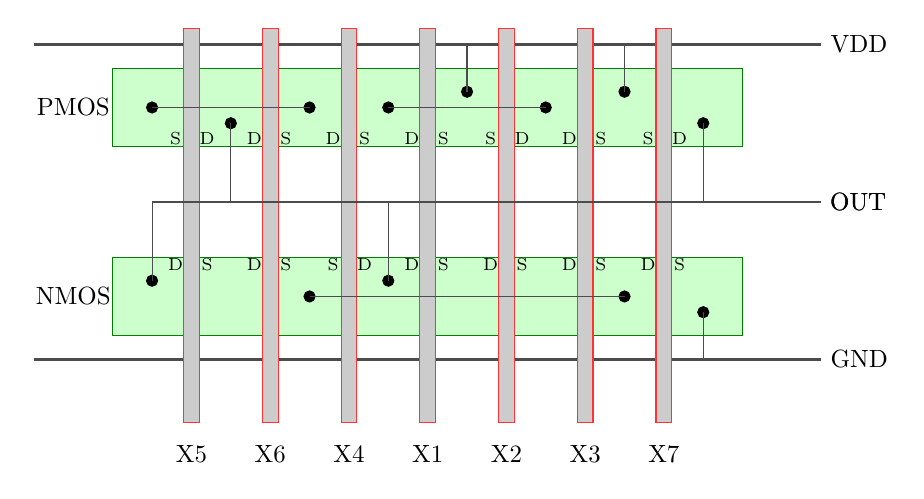
\begin{tikzpicture}[scale=1, every node/.style={scale=0.9}]

% Define styles for layers
\tikzstyle{nwell} = [draw=blue!40, fill=blue!10]
\tikzstyle{poly} = [draw=red!80, fill=gray!40]
\tikzstyle{diffusion} = [draw=green!50!black, fill=green!20]
\tikzstyle{metal} = [draw=black!70, fill=gray!30]
\tikzstyle{contact} = [draw=black, fill=black]

% Draw power rails
\draw[metal, thick] (0,4) -- (10,4) node[right] {VDD};
\draw[metal, thick] (0,0) -- (10,0) node[right] {GND};

% Draw PMOS diffusion region
\draw[diffusion] (1,2.7) rectangle (9,3.7);
\node at (0.5,3.2) {PMOS};

% Draw NMOS diffusion region
\draw[diffusion] (1,0.3) rectangle (9,1.3);
\node at (0.5,0.8) {NMOS};

% Example polysilicon gates
\foreach \x in {2,3,4,5,6,7,8} {
%   \draw[poly] (\x,-0.0) rectangle (\x,4.2);
%   \draw[poly] (\x,-0.8) -- (\x,4.2);
  \draw[poly] (\x+0.1,-0.8) rectangle (\x-0.1,4.2);

%   \filldraw[contact] (\x,0.8) circle (0.05);
%   \filldraw[contact] (\x,3.2) circle (0.05);
}

% \draw[poly] (2.1,-0.8) rectangle (1.9,4.2);

% % PMOS Contacts
% For OUT
\filldraw[contact] (2.5,3.0) circle (0.07);
\filldraw[contact] (8.5,3.0) circle (0.07);
\draw[metal] (2.5,3.0) -- (2.5,2);
\draw[metal] (8.5,3.0) -- (8.5,2);
\draw[metal] (2.5,2) -- (10,2) node[right] {OUT};
% For Node 3
\filldraw[contact] (1.5,3.2) circle (0.07);
\filldraw[contact] (3.5,3.2) circle (0.07);
\draw[metal] (1.5,3.2) -- (3.5,3.2);
% For Node 2
\filldraw[contact] (4.5,3.2) circle (0.07);
\filldraw[contact] (6.5,3.2) circle (0.07);
\draw[metal] (4.5,3.2) -- (6.5,3.2);
% For VDD
\filldraw[contact] (5.5,3.4) circle (0.07);
\filldraw[contact] (7.5,3.4) circle (0.07);
\draw[metal] (5.5,3.4) -- (5.5,4);
\draw[metal] (7.5,3.4) -- (7.5,4);

\node at (1.8,2.8) {\scriptsize S};
\node at (2.2,2.8) {\scriptsize D};

\node at (2.8,2.8) {\scriptsize D};
\node at (3.2,2.8) {\scriptsize S};

\node at (3.8,2.8) {\scriptsize D};
\node at (4.2,2.8) {\scriptsize S};

\node at (4.8,2.8) {\scriptsize D};
\node at (5.2,2.8) {\scriptsize S};

\node at (5.8,2.8) {\scriptsize S};
\node at (6.2,2.8) {\scriptsize D};

\node at (6.8,2.8) {\scriptsize D};
\node at (7.2,2.8) {\scriptsize S};

\node at (7.8,2.8) {\scriptsize S};
\node at (8.2,2.8) {\scriptsize D};




% NMOS Contacts
% For OUT
\filldraw[contact] (1.5,1.0) circle (0.07);
\filldraw[contact] (4.5,1.0) circle (0.07);
\draw[metal] (1.5,1.0) -- (1.5,2);
\draw[metal] (4.5,1.0) -- (4.5,2);
\draw[metal] (1.5,2) -- (10,2) node[right] {OUT};
% For Node 5
% For Node 6
% For Node 7
% For Node 8
\filldraw[contact] (3.5,0.8) circle (0.07);
\filldraw[contact] (7.5,0.8) circle (0.07);
\draw[metal] (3.5,0.8) -- (7.5,0.8);
% For GND
\filldraw[contact] (8.5,0.6) circle (0.07);
\draw[metal] (8.5,0.6) -- (8.5,0);

\node at (1.8,1.2) {\scriptsize D};
\node at (2.2,1.2) {\scriptsize S};

\node at (2.8,1.2) {\scriptsize D};
\node at (3.2,1.2) {\scriptsize S};

\node at (3.8,1.2) {\scriptsize S};
\node at (4.2,1.2) {\scriptsize D};

\node at (4.8,1.2) {\scriptsize D};
\node at (5.2,1.2) {\scriptsize S};

\node at (5.8,1.2) {\scriptsize D};
\node at (6.2,1.2) {\scriptsize S};

\node at (6.8,1.2) {\scriptsize D};
\node at (7.2,1.2) {\scriptsize S};

\node at (7.8,1.2) {\scriptsize D};
\node at (8.2,1.2) {\scriptsize S};




% Input labels
\node at (2,-1.2) {X5};
\node at (3,-1.2) {X6};
\node at (4,-1.2) {X4};
\node at (5,-1.2) {X1};
\node at (6,-1.2) {X2};
\node at (7,-1.2) {X3};
\node at (8,-1.2) {X7};

% % VDD and GND contacts
% \foreach \x in {1,7} {
%   \filldraw[contact] (\x,3.7) circle (0.07);
%   \filldraw[contact] (\x,0.3) circle (0.07);
% }

% Metal connections (example)
% \draw[metal, thick] (3,3.7) -- (3,4); % PMOS to VDD
% \draw[metal, thick] (4,0.3) -- (4,0); % NMOS to GND
% \draw[metal, thick] (4,3.7) -- (4.5,3.7) -- (4.5,0.3) -- (4,0.3); % output path

% Output label
% \node at (4.5,2) {Y (output)};
% \filldraw[contact] (4.5,3.7) circle (0.07);
% \filldraw[contact] (4.5,0.3) circle (0.07);

\end{tikzpicture}
\caption{Stick diagram according to Euler's Path.}
\label{fig:stick}
\end{figure}

\section{Electric Drawing}
\autoref{fig:fig:stick} shows drawing of the circuit by using Electric, $.jelib$ file is also attached to this homework.
\begin{figure}[ht!]
\centering
 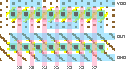
\includegraphics[width=0.7\textwidth]{7_input_function.pdf}
 \caption{Drawing output from Electric}
\label{fig:fig:stick}

\end{figure}


\end{document}






